%*************************************************************************

% Note that the a4paper option is mainly intended so that authors in
% countries using A4 can easily print to A4 and see how their papers will
% look in print - the typesetting of the document will not typically be
% affected with changes in paper size (but the bottom and side margins will).
% Use the testflow package mentioned above to verify correct handling of
% both paper sizes by the user's LaTeX system.
%
% Also note that the "draftcls" or "draftclsnofoot", not "draft", option
% should be used if it is desired that the figures are to be displayed in
% draft mode.
%
\documentclass[journal]{IEEEtran}
%
% If IEEEtran.cls has not been installed into the LaTeX system files,
% manually specify the path to it like:
% \documentclass[journal]{../sty/IEEEtran}





% Some very useful LaTeX packages include:
% (uncomment the ones you want to load)


% *** MISC UTILITY PACKAGES ***
%
%\usepackage{ifpdf}
% Heiko Oberdiek's ifpdf.sty is very useful if you need conditional
% compilation based on whether the output is pdf or dvi.
% usage:
% \ifpdf
%   % pdf code
% \else
%   % dvi code
% \fi
% The latest version of ifpdf.sty can be obtained from:
% http://www.ctan.org/tex-archive/macros/latex/contrib/oberdiek/
% Also, note that IEEEtran.cls V1.7 and later provides a builtin
% \ifCLASSINFOpdf conditional that works the same way.
% When switching from latex to pdflatex and vice-versa, the compiler may
% have to be run twice to clear warning/error messages.






% *** CITATION PACKAGES ***
%
%\usepackage{cite}
% cite.sty was written by Donald Arseneau
% V1.6 and later of IEEEtran pre-defines the format of the cite.sty package
% \cite{} output to follow that of IEEE. Loading the cite package will
% result in citation numbers being automatically sorted and properly
% "compressed/ranged". e.g., [1], [9], [2], [7], [5], [6] without using
% cite.sty will become [1], [2], [5]--[7], [9] using cite.sty. cite.sty's
% \cite will automatically add leading space, if needed. Use cite.sty's
% noadjust option (cite.sty V3.8 and later) if you want to turn this off.
% cite.sty is already installed on most LaTeX systems. Be sure and use
% version 4.0 (2003-05-27) and later if using hyperref.sty. cite.sty does
% not currently provide for hyperlinked citations.
% The latest version can be obtained at:
% http://www.ctan.org/tex-archive/macros/latex/contrib/cite/
% The documentation is contained in the cite.sty file itself.




\usepackage[pdftex]{graphicx}

\usepackage{float}
  % 
  % declare the path(s) where your graphic files are
\graphicspath{{../pdf/}{../jpeg/}}
  % and their extensions so you won't have to specify these with
  % every instance of \includegraphics
\DeclareGraphicsExtensions{.pdf,.jpeg,.png}





% *** MATH PACKAGES ***
%
%\usepackage[cmex10]{amsmath}
% A popular package from the American Mathematical Society that provides
% many useful and powerful commands for dealing with mathematics. If using
% it, be sure to load this package with the cmex10 option to ensure that
% only type 1 fonts will utilized at all point sizes. Without this option,
% it is possible that some math symbols, particularly those within
% footnotes, will be rendered in bitmap form which will result in a
% document that can not be IEEE Xplore compliant!
%
% Also, note that the amsmath package sets \interdisplaylinepenalty to 10000
% thus preventing page breaks from occurring within multiline equations. Use:
%\interdisplaylinepenalty=2500
% after loading amsmath to restore such page breaks as IEEEtran.cls normally
% does. amsmath.sty is already installed on most LaTeX systems. The latest
% version and documentation can be obtained at:
% http://www.ctan.org/tex-archive/macros/latex/required/amslatex/math/





% *** SPECIALIZED LIST PACKAGES ***
%
%\usepackage{algorithmic}
% algorithmic.sty was written by Peter Williams and Rogerio Brito.
% This package provides an algorithmic environment fo describing algorithms.
% You can use the algorithmic environment in-text or within a figure
% environment to provide for a floating algorithm. Do NOT use the algorithm
% floating environment provided by algorithm.sty (by the same authors) or
% algorithm2e.sty (by Christophe Fiorio) as IEEE does not use dedicated
% algorithm float types and packages that provide these will not provide
% correct IEEE style captions. The latest version and documentation of
% algorithmic.sty can be obtained at:
% http://www.ctan.org/tex-archive/macros/latex/contrib/algorithms/
% There is also a support site at:
% http://algorithms.berlios.de/index.html
% Also of interest may be the (relatively newer and more customizable)
% algorithmicx.sty package by Szasz Janos:
% http://www.ctan.org/tex-archive/macros/latex/contrib/algorithmicx/




% *** ALIGNMENT PACKAGES ***
%
%\usepackage{array}
% Frank Mittelbach's and David Carlisle's array.sty patches and improves
% the standard LaTeX2e array and tabular environments to provide better
% appearance and additional user controls. As the default LaTeX2e table
% generation code is lacking to the point of almost being broken with
% respect to the quality of the end results, all users are strongly
% advised to use an enhanced (at the very least that provided by array.sty)
% set of table tools. array.sty is already installed on most systems. The
% latest version and documentation can be obtained at:
% http://www.ctan.org/tex-archive/macros/latex/required/tools/


%\usepackage{mdwmath}
%\usepackage{mdwtab}
% Also highly recommended is Mark Wooding's extremely powerful MDW tools,
% especially mdwmath.sty and mdwtab.sty which are used to format equations
% and tables, respectively. The MDWtools set is already installed on most
% LaTeX systems. The lastest version and documentation is available at:
% http://www.ctan.org/tex-archive/macros/latex/contrib/mdwtools/


% IEEEtran contains the IEEEeqnarray family of commands that can be used to
% generate multiline equations as well as matrices, tables, etc., of high
% quality.


%\usepackage{eqparbox}
% Also of notable interest is Scott Pakin's eqparbox package for creating
% (automatically sized) equal width boxes - aka "natural width parboxes".
% Available at:
% http://www.ctan.org/tex-archive/macros/latex/contrib/eqparbox/





% *** SUBFIGURE PACKAGES ***
%\usepackage[tight,footnotesize]{subfigure}
% subfigure.sty was written by Steven Douglas Cochran. This package makes it
% easy to put subfigures in your figures. e.g., "Figure 1a and 1b". For IEEE
% work, it is a good idea to load it with the tight package option to reduce
% the amount of white space around the subfigures. subfigure.sty is already
% installed on most LaTeX systems. The latest version and documentation can
% be obtained at:
% http://www.ctan.org/tex-archive/obsolete/macros/latex/contrib/subfigure/
% subfigure.sty has been superceeded by subfig.sty.



%\usepackage[caption=false]{caption}
%\usepackage[font=footnotesize]{subfig}
% subfig.sty, also written by Steven Douglas Cochran, is the modern
% replacement for subfigure.sty. However, subfig.sty requires and
% automatically loads Axel Sommerfeldt's caption.sty which will override
% IEEEtran.cls handling of captions and this will result in nonIEEE style
% figure/table captions. To prevent this problem, be sure and preload
% caption.sty with its "caption=false" package option. This is will preserve
% IEEEtran.cls handing of captions. Version 1.3 (2005/06/28) and later 
% (recommended due to many improvements over 1.2) of subfig.sty supports
% the caption=false option directly:
%\usepackage[caption=false,font=footnotesize]{subfig}
%
% The latest version and documentation can be obtained at:
% http://www.ctan.org/tex-archive/macros/latex/contrib/subfig/
% The latest version and documentation of caption.sty can be obtained at:
% http://www.ctan.org/tex-archive/macros/latex/contrib/caption/




% *** FLOAT PACKAGES ***
%
%\usepackage{fixltx2e}
% fixltx2e, the successor to the earlier fix2col.sty, was written by
% Frank Mittelbach and David Carlisle. This package corrects a few problems
% in the LaTeX2e kernel, the most notable of which is that in current
% LaTeX2e releases, the ordering of single and double column floats is not
% guaranteed to be preserved. Thus, an unpatched LaTeX2e can allow a
% single column figure to be placed prior to an earlier double column
% figure. The latest version and documentation can be found at:
% http://www.ctan.org/tex-archive/macros/latex/base/



%\usepackage{stfloats}
% stfloats.sty was written by Sigitas Tolusis. This package gives LaTeX2e
% the ability to do double column floats at the bottom of the page as well
% as the top. (e.g., "\begin{figure*}[!b]" is not normally possible in
% LaTeX2e). It also provides a command:
%\fnbelowfloat
% to enable the placement of footnotes below bottom floats (the standard
% LaTeX2e kernel puts them above bottom floats). This is an invasive package
% which rewrites many portions of the LaTeX2e float routines. It may not work
% with other packages that modify the LaTeX2e float routines. The latest
% version and documentation can be obtained at:
% http://www.ctan.org/tex-archive/macros/latex/contrib/sttools/
% Documentation is contained in the stfloats.sty comments as well as in the
% presfull.pdf file. Do not use the stfloats baselinefloat ability as IEEE
% does not allow \baselineskip to stretch. Authors submitting work to the
% IEEE should note that IEEE rarely uses double column equations and
% that authors should try to avoid such use. Do not be tempted to use the
% cuted.sty or midfloat.sty packages (also by Sigitas Tolusis) as IEEE does
% not format its papers in such ways.


%\ifCLASSOPTIONcaptionsoff
%  \usepackage[nomarkers]{endfloat}
% \let\MYoriglatexcaption\caption
% \renewcommand{\caption}[2][\relax]{\MYoriglatexcaption[#2]{#2}}
%\fi
% endfloat.sty was written by James Darrell McCauley and Jeff Goldberg.
% This package may be useful when used in conjunction with IEEEtran.cls'
% captionsoff option. Some IEEE journals/societies require that submissions
% have lists of figures/tables at the end of the paper and that
% figures/tables without any captions are placed on a page by themselves at
% the end of the document. If needed, the draftcls IEEEtran class option or
% \CLASSINPUTbaselinestretch interface can be used to increase the line
% spacing as well. Be sure and use the nomarkers option of endfloat to
% prevent endfloat from "marking" where the figures would have been placed
% in the text. The two hack lines of code above are a slight modification of
% that suggested by in the endfloat docs (section 8.3.1) to ensure that
% the full captions always appear in the list of figures/tables - even if
% the user used the short optional argument of \caption[]{}.
% IEEE papers do not typically make use of \caption[]'s optional argument,
% so this should not be an issue. A similar trick can be used to disable
% captions of packages such as subfig.sty that lack options to turn off
% the subcaptions:
% For subfig.sty:
% \let\MYorigsubfloat\subfloat
% \renewcommand{\subfloat}[2][\relax]{\MYorigsubfloat[]{#2}}
% For subfigure.sty:
% \let\MYorigsubfigure\subfigure
% \renewcommand{\subfigure}[2][\relax]{\MYorigsubfigure[]{#2}}
% However, the above trick will not work if both optional arguments of
% the \subfloat/subfig command are used. Furthermore, there needs to be a
% description of each subfigure *somewhere* and endfloat does not add
% subfigure captions to its list of figures. Thus, the best approach is to
% avoid the use of subfigure captions (many IEEE journals avoid them anyway)
% and instead reference/explain all the subfigures within the main caption.
% The latest version of endfloat.sty and its documentation can obtained at:
% http://www.ctan.org/tex-archive/macros/latex/contrib/endfloat/
%
% The IEEEtran \ifCLASSOPTIONcaptionsoff conditional can also be used
% later in the document, say, to conditionally put the References on a 
% page by themselves.





% *** PDF, URL AND HYPERLINK PACKAGES ***
%
%\usepackage{url}
% url.sty was written by Donald Arseneau. It provides better support for
% handling and breaking URLs. url.sty is already installed on most LaTeX
% systems. The latest version can be obtained at:
% http://www.ctan.org/tex-archive/macros/latex/contrib/misc/
% Read the url.sty source comments for usage information. Basically,
% \url{my_url_here}.





% *** Do not adjust lengths that control margins, column widths, etc. ***
% *** Do not use packages that alter fonts (such as pslatex).         ***
% There should be no need to do such things with IEEEtran.cls V1.6 and later.
% (Unless specifically asked to do so by the journal or conference you plan
% to submit to, of course. )


% correct bad hyphenation here
\hyphenation{op-tical net-works semi-conduc-tor}


\begin{document}
%
% paper title
% can use linebreaks \\ within to get better formatting as desired
\title{Sparky - Gesture Based Home Automation Application}
%
%
% author names and IEEE memberships
% note positions of commas and nonbreaking spaces ( ~ ) LaTeX will not break
% a structure at a ~ so this keeps an author's name from being broken across
% two lines.
% use \thanks{} to gain access to the first footnote area
% a separate \thanks must be used for each paragraph as LaTeX2e's \thanks
% was not built to handle multiple paragraphs
%

\author{Gary~Graham,
        Jia~Ming~(Anson)~Liang,
        and~Jyotheeswar~Arvind~M% <-this % stops a space
}

% note the % following the last \IEEEmembership and also \thanks - 
% these prevent an unwanted space from occurring between the last author name
% and the end of the author line. i.e., if you had this:
% 
% \author{....lastname \thanks{...} \thanks{...} }
%                     ^------------^------------^----Do not want these spaces!
%
% a space would be appended to the last name and could cause every name on that
% line to be shifted left slightly. This is one of those "LaTeX things". For
% instance, "\textbf{A} \textbf{B}" will typeset as "A B" not "AB". To get
% "AB" then you have to do: "\textbf{A}\textbf{B}"
% \thanks is no different in this regard, so shield the last } of each \thanks
% that ends a line with a % and do not let a space in before the next \thanks.
% Spaces after \IEEEmembership other than the last one are OK (and needed) as
% you are supposed to have spaces between the names. For what it is worth,
% this is a minor point as most people would not even notice if the said evil
% space somehow managed to creep in.



% The paper headers
\markboth{ECE1780: Advance Mobile UI Project Report}%
{Shell \MakeLowercase{\textit{et al.}}: Bare Demo of IEEEtran.cls for Journals}
% The only time the second header will appear is for the odd numbered pages
% after the title page when using the twoside option.
% 
% *** Note that you probably will NOT want to include the author's ***
% *** name in the headers of peer review papers.                   ***
% You can use \ifCLASSOPTIONpeerreview for conditional compilation here if
% you desire.




% If you want to put a publisher's ID mark on the page you can do it like
% this:
%\IEEEpubid{0000--0000/00\$00.00~\copyright~2007 IEEE}
% Remember, if you use this you must call \IEEEpubidadjcol in the second
% column for its text to clear the IEEEpubid mark.



% use for special paper notices
%\IEEEspecialpapernotice{(Invited Paper)}




% make the title area
\maketitle


\begin{abstract}
%\boldmath
Traditional home automation applications mainly use buttons on the mobile phone touch display to toggle the state of home devices. These applications usually require users to navigate through clusters of buttons to control the specific device. Most users would rather flip the switches on their home wall to toggle the specific devices instead of going into their applications to find the correct button. We built an Android application to utilize motion gestures to control the home devices. This will eliminate the process of users trying to find the correct button on the screen. With our application, users can toggle a specific device by simply performing a unique gesture with their mobile phone. Our application connects to a Spark Core, which we use for our home automation system. Spark Core is an Arduino-compatible Wi-Fi enabled device that can be used for developing internet-connected hardware. This device enables our application to let users control their home devices anywhere with internet access.


\end{abstract}
% IEEEtran.cls defaults to using nonbold math in the Abstract.
% This preserves the distinction between vectors and scalars. However,
% if the journal you are submitting to favors bold math in the abstract,
% then you can use LaTeX's standard command \boldmath at the very start
% of the abstract to achieve this. Many IEEE journals frown on math
% in the abstract anyway.

% Note that keywords are not normally used for peerreview papers.
\begin{IEEEkeywords}
Android, Arduino, Gesture, Home Automation, Spark Core.
\end{IEEEkeywords}






% For peer review papers, you can put extra information on the cover
% page as needed:
% \ifCLASSOPTIONpeerreview
% \begin{center} \bfseries EDICS Category: 3-BBND \end{center}
% \fi
%
% For peerreview papers, this IEEEtran command inserts a page break and
% creates the second title. It will be ignored for other modes.
\IEEEpeerreviewmaketitle



\section{Introduction}
% The very first letter is a 2 line initial drop letter followed
% by the rest of the first word in caps.
% 
% form to use if the first word consists of a single letter:
% \IEEEPARstart{A}{demo} file is ....
% 
% form to use if you need the single drop letter followed by
% normal text (unknown if ever used by IEEE):
% \IEEEPARstart{A}{}demo file is ....
% 
% Some journals put the first two words in caps:
% \IEEEPARstart{T}{his demo} file is ....
% 
% Here we have the typical use of a "T" for an initial drop letter
% and "HIS" in caps to complete the first word.
\IEEEPARstart{W}{}ith the development of our application, we wanted to address what we believe to be an up and coming problem in the world of Internet of Things (IoT). In the home automation space, there are many manufacturers. Each of these manufacturers typically develop applications to support their proprietary devices. However, a quick search on the mobile applications stores show that the UI and usability of these applications leave much to be desired[2]. Cluttered interfaces with no regard to user experience abound. With this in mind, our goal was to create a home automation application that is not only more aesthetically pleasing, but also more functional.

Traditional home automation applications have stuck to the tried and tested method of utilizing buttons inside an application, typically on a mobile device, to toggle the state of devices at home. However, we have many more ways to interact with our mobile devices than simple taps. The overarching goal for home automation is to make the experience seamless for users. If it is not faster or more convenient to use your mobile phone to toggle a device, then why bother? If users want to turn off a light, and it takes them two seconds to take out their phone, 5 seconds to scroll over to the application and open it, 1 second for it to load, and 1 second for users to tap on the correct button; they have taken 9-10 seconds to do something they could have done in the same time by simply standing up and going to flip the switch manually. We believe that using gesture-based triggers, combined with widgets, users can achieve a more satisfactory experience, while reducing the time it takes to actually perform the task at hand. 

For the purpose of demonstration, we will only use the 3-Axis accelerometer data available in our Android device to perform gesture recognition. The algorithm we use is a simple discrete time series data matching algorithm called Dynamic Time Warping (DTW). It should be noted that gesture recognition is non-trivial and high degrees of accuracy will require using advanced machine learning techniques. 

This paper gives an overview of our application, explaining how we setup and connect to the Spark Core home automation system. This paper also explains how we implement our gesture based cognition to control a Spark Core and show results of user experience tests.

\section{Overview of the application}
The goal of this application is quite straightforward; improve the current state of home automation user interaction. To perform this, we go about it in three ways. Firstly, we improve the communications between mobile and the physical devices at home. Secondly, we implement gesture recognition as a device-toggling mechanism. Third, we build our prototype using publically available devices, which will allow users to extend our work.  

The prototype of the device involves the following:
\begin{enumerate}
	\item Spark Core
	\item Relay Board
	\item 2x Electrical Outlet
	\item Android Device
\end{enumerate}

Users can plug any of their devices into either one outlet or the other. Then, within the android application, they can toggle the power to each of the outlets individually, and become informed if the status of one of the outlets changes.

For user interaction, we have decided on a multi-faceted approach. The novelty of the application comes from our gesture recognition system which allows the mobile device to register gestures even while the phone is asleep. This in turn toggles power to the devices.  Beyond this, we have also implemented widgets, which allows users to define their own interface on their home screens. For example, you can split half your home screen between two widgets for easy access to the functionality, even when not inside the app. Furthermore, we allow users to toggle devices in the traditional sense, using buttons inside the application itself. 

To begin with, we discuss the communications method used. To build our prototype, we used a Spark Core[1]. The device exposes a REpresentational State Transfer(REST) API to anybody who has the credentials, and operates over a Wi-Fi network. The advantage of this is that it is extremely light-weight, and requires no proprietary technology. The Spark Core, being an Arduino-based microcontroller, also allows us to quickly and remotely modify the code running on it. 

In this section we give an overview of our Android application prototype, Sparky. We omit low-level implementation details in favour of providing a high-level overview of the interactions. In order to allow the mobile phone to communicate, we have written a communications library that allows us to interact with the Spark Core. It is upon this interaction which the backbone of the application rests. Whenever an intent to toggle is registered, whether by gesture recognition or otherwise, a call is made to the library, which handles request and response. Since we have many UI elements indicating the status of the device(in-app, multiple widgets), we use the observer pattern to handle notifying all listeners as to the status of the device. For the in-app and widget UI, we use minimalistic icons that represent the devices they are toggling. This declutters the interface and provides an intuitive idea of how to use the appplication. Fig. \ref{fig1} shows the overall basic usage of the application.

\begin{figure}[!t]
\centering
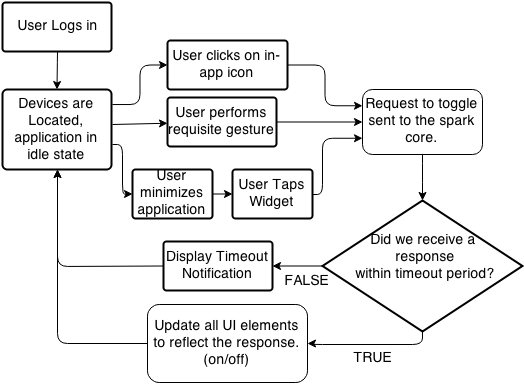
\includegraphics[width=3.5in]{Workflow.png}
\caption{Application workflow diagram}
\label{fig1}
\end{figure}



There are equivalent workflows for other tasks, for example changing the current gesture, but we omit them here due to brevity requirements. 

\section{Gesture Recognition}

Our application uses the DTW algorithm to do gesture recognition. DTW was originally developed for speech recognition by measuring the similarity between two discrete time series data. Instead of speech, we compare accelerometer data for gesture recognition. DTW is relatively simple to implement and it works for simple gestures. Below is a pseudo-code algorithm for DTW:\\
\noindent 
	double DTW(double 01[1...T1], double O2[1...T2])\\
 	\hspace*{0.25cm}declare double DTW[0...T1, 0....T2]\\
 	\hspace*{0.25cm}declare integer i, j\\
 	\hspace*{0.25cm}for i:=1 to T1\\
 	\hspace*{0.5cm}DTW[i,0] := positive infinity\\
 	\hspace*{0.25cm}for j:=1 to T2\\
 	\hspace*{0.25cm}DTW[0,j] := positive infinity\\
 	\hspace*{0.25cm}DTW[0,0] := 0\\
 	\hspace*{0.25cm}for i:=1 to T1\\
 	\hspace*{0.5cm}for j:= 1 to T2\\
 	\hspace*{0.75cm}DTW[i,j] := distance(O1[i], O2[j]) +\\
 	\hspace*{1cm}minimum(DTW[i-1,j]), DTW[i,j-1], DTW[i-1,j-1])\\
 	\hspace*{0.25cm}return DTW[T1,T2]

Since the data reading is in 3-Dimensional space, we treat each time interval reading as a 3-Dimensional point. The distance function we use in the pseudo code takes the norm between the two points. 

Before gesture recognition, we train a gesture by obtaining and storing 32 discrete accelerometer data. This accelerometer data combined with a gesture label form a gesture object. Our application, by default, contains two predefined gestures: Bump Front and Bump Left. We choose these two gestures as default because it is very simple for another person to repeat the movement and it is unique enough that when someone puts their phone in their pocket for example, they will not accidentally trigger the gesture.

\begin{figure}[H]
\centering
\includegraphics[width=1.5in]{S1.jpg}
\caption{Default gestures selection page for Sparky}
\label{fig2}
\end{figure}


Bump Front in fig. \ref{fig2} is defined by holding the device straight, tilting it forward by 90 degrees and back to the original position within 2 seconds. Bump Left is defined similarly, tilting the phone to the left by 90 degrees and back to the original position within 2 seconds. Users have the option of creating their own custom gestures.

Once users select the gesture for a particular device, and make their preference about listening to gestures being performed in the background, the application listens to the accelerometer data. This data is compared with the stored gestures using the DTW algorithm. DTW will return the distance for every stored gestures. This distance indicates how similar the two gestures are, with a smaller distance indicating they are very similar and vice versa. We take the geture with the smallest distance as the recognized gesture. 

DTW allows some variance in gesture motion and speed when a person tries to repeat the gesture they trained. The variance is controlled by a threshold variable in our program. We find that small variance will allow us to get high percentage of true positive recognition but we realize that it takes multiple tries for users to re-do the same gesture they trained. On the other hand, large variance will allow users to easily get their gesture recognized but will also have high chance of getting false positive recognition. 

\begin{figure}[H]
\centering
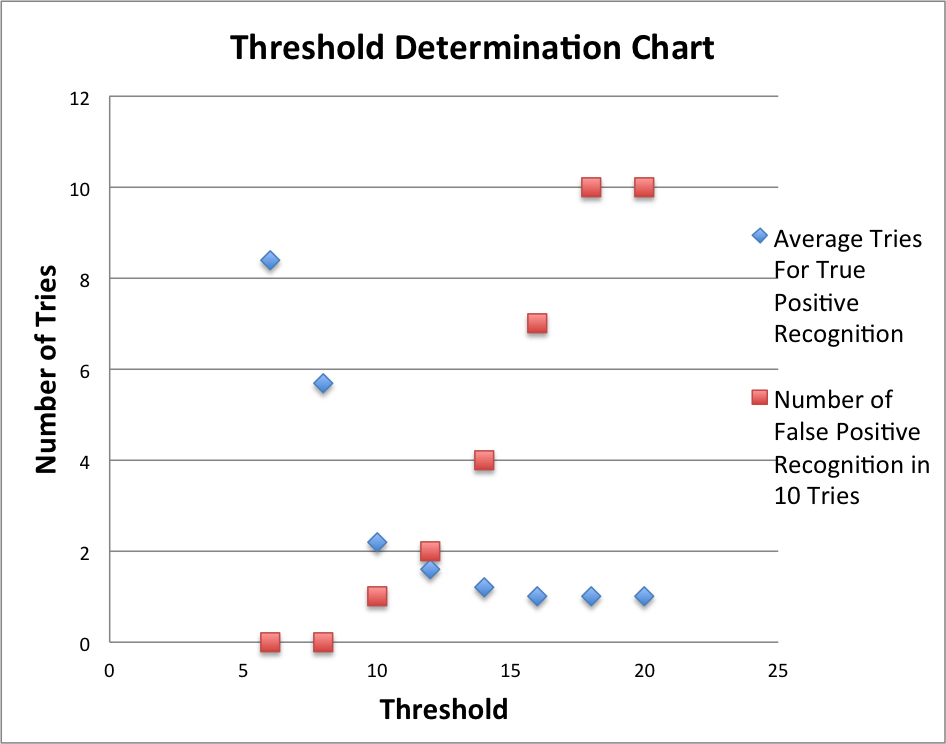
\includegraphics[width=3in]{threshold.png}
\caption{Chart used to determining distance threshold}
\label{fig3}
\end{figure}

	We set the distance threshold by experiementation. We try to set the threshold so that we minimize both the number of tries to get true positive recognition and the number of accidental false positive recognition. In fig. \ref{fig3}, the diamond scatter plot is the average number of tries to get a proper gesture recognized. We have a person train their own gesture and try to reproduce the same gesture at different thresholds multiple times. We then take the average of this set to the threshold. The square scatter plot is having a person doing 10 random gestures and see how many gestures will get recognized (these are false positive results). We can see in fig. \ref{fig3} that the ideal threshold value is around 12.  

 


\section{User Experience Tests}

The application was tested by 17 users aged between 21-27 and we obtained their feedback. The participants of the testing consisted of mainly graduate students with a strong technical background. 

\subsection{Methodology}

The participants tested the application individually and not more than two participants were in the testing room at a particular point of time. The participants were initially briefed about the overall idea of the application. The team demonstrated the functioning of the application first and explained how to perform the default gestures. Then the participants were given access to the mobile device on which the application is running. The participants tested the entire functionality of the application including changing the assigned gestures and creating their own custom gestures. There was no set time limit for the participants to use the application. Upon their stating that they have completed testing the application, they were directed to fill in an online feedback form. The questions on the feedback form were structured to get the users' rating on factors such as the intuitiveness of the application, their comfort using the default gestures, their willingness/interest in adapting such technology to control home appliances using our mobile application.

\subsection{User Feedback}

Users submitted their feedback and comments online. Users also provided their consent on the form before submitting their feedback.

Some comments from the users are: ``Takes a bit of trial and error to figure out the default gestures. They seem pretty sensitive. '', ``The default gestures are good, but , take some time to adjust to the user's personal way of doing these gestures. So, even before using the default gestures, learning  these from the user might make this a bit easier'',``why does every single thing have to be internet connected nowadays. Dont track any usage data!'' etc. 

\subsection{Inference}

The application experience rating on a scale of 10 was found to have a mean of 8.58,  and median of 9. Although users rated the default gesture experience at a mean of 7.88 and median of 8, about 53\% of the users needed multiple attempts to get accustomed to the way the default gestures have been defined. This is attested by the rating on the ease of figuring out the default gesture, with a mean of 7.5 and median of 8. Since the data obtained when a gesture is performed is reliant on orientation and the starting position at the time of doing the gesture, users needed practice before being comfortable. Once they learnt the default gestures, the usability of the application became smooth. The application's intuitiveness received a mean rating of 8.11 with a median of 8. On being comfortable to use the application in a real life setting, users gave a positive 70.5\% yes. It is interesting to note that 76.47\% of the users were comfortable using our application to control household devices, albeit this can be due to the users being in the 21-27 age group and most users being from a technical background. 

\begin{figure}[!t]
\centering
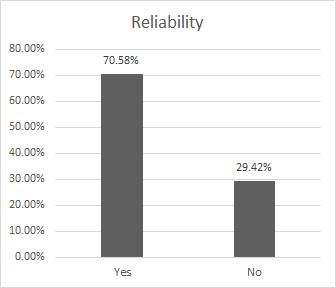
\includegraphics[width=3in]{R1.jpg}
\caption{C1}
\label{fig2}
\end{figure}
\begin{figure}[!t]
\centering
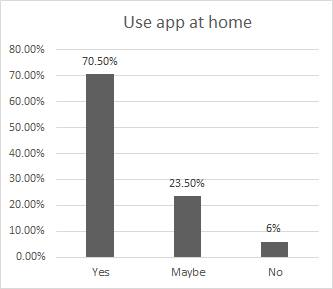
\includegraphics[width=3in]{R2.jpg}
\caption{C2}
\label{fig2}
\end{figure}
\begin{figure}[!t]
\centering
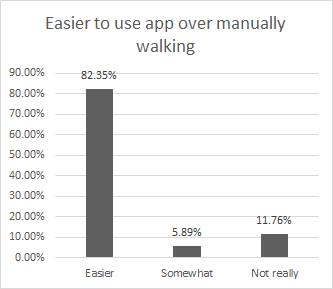
\includegraphics[width=3in]{R3.jpg}
\caption{C3}
\label{fig2}
\end{figure}
\begin{figure}[!t]
\centering
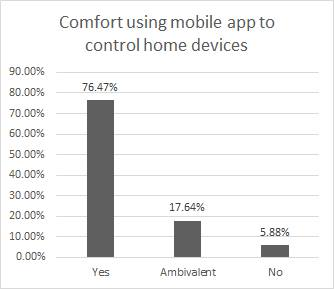
\includegraphics[width=3in]{R4.jpg}
\caption{C4}
\label{fig2}
\end{figure}
\begin{figure}[!t]
\centering
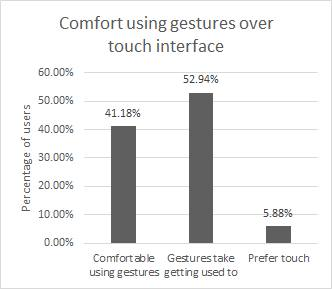
\includegraphics[width=3in]{R5.jpg}
\caption{C5}
\label{fig2}
\end{figure}
\begin{figure}[!t]
\centering
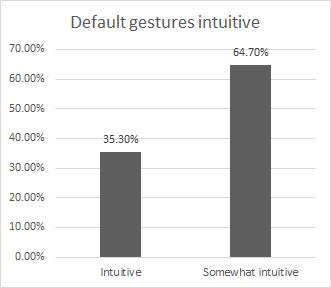
\includegraphics[width=3in]{R7.jpg}
\caption{C6}
\label{fig2}
\end{figure}
\begin{figure}[!t]
\centering
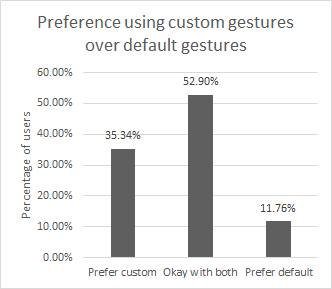
\includegraphics[width=3in]{R6.jpg}
\caption{C7}
\label{fig2}
\end{figure}


\section{Future Work}
We aim to improve our application in the future by providing an interface for multiple Spark Cores to be connected to our application. Functionality to add more devices, with corresponding images, are also targeted. 

We aim to improve the accuracy of the gesture recognition by incorporating the 3-Axis gyrometer. We would also want to have an option for users to utilize the magnetometer to control multiple devices with the same gesture but perform the gesture at a particular direction. 

DTW is an effective algorithm when the gesture is a simple motion. It allows small variation in speed and motion. However, our user feedback results show that the default gestures are minimally comfortable because the algorithm generally performs poorly when the moving rate and motion have a large variation; as is common among different users. Also, with more complicated gestures DTW will not work effectively. One alternative is to do gesture recognition is Hidden Markov Models (a machine learning technique). This technique is better because it uses knowledge in probability and stastics to account for larger variation of speed and motion, but still retain the accuracy of recognizing gestures. 

We also aim to test the application among a wider audience to observe how much this technology/application is acceptable to the greater populace.
\section{Conclusion}




\newpage
\begin{thebibliography}{1}

\bibitem{IEEEhowto:kopka}
H.~Kopka and P.~W. Daly, \emph{A Guide to \LaTeX}, 3rd~ed.\hskip 1em plus
  0.5em minus 0.4em\relax Harlow, England: Addison-Wesley, 1999.
https://www.spark.io/
https://play.google.com/store/apps/details?id=com.webmtn.android.app

\end{thebibliography}































\if
\hfill mds
 
\hfill January 11, 2007


% needed in second column of first page if using \IEEEpubid
%\IEEEpubidadjcol

\subsubsection{Subsubsection Heading Here}
Subsubsection text here.


% An example of a floating figure using the graphicx package.
% Note that \label must occur AFTER (or within) \caption.
% For figures, \caption should occur after the \includegraphics.
% Note that IEEEtran v1.7 and later has special internal code that
% is designed to preserve the operation of \label within \caption
% even when the captionsoff option is in effect. However, because
% of issues like this, it may be the safest practice to put all your
% \label just after \caption rather than within \caption{}.
%
% Reminder: the "draftcls" or "draftclsnofoot", not "draft", class
% option should be used if it is desired that the figures are to be
% displayed while in draft mode.
%
%\begin{figure}[!t]
%\centering
%\includegraphics[width=2.5in]{myfigure}
% where an .eps filename suffix will be assumed under latex, 
% and a .pdf suffix will be assumed for pdflatex; or what has been declared
% via \DeclareGraphicsExtensions.
%\caption{Simulation Results}
%\label{fig_sim}
%\end{figure}

% Note that IEEE typically puts floats only at the top, even when this
% results in a large percentage of a column being occupied by floats.


% An example of a double column floating figure using two subfigures.
% (The subfig.sty package must be loaded for this to work.)
% The subfigure \label commands are set within each subfloat command, the
% \label for the overall figure must come after \caption.
% \hfil must be used as a separator to get equal spacing.
% The subfigure.sty package works much the same way, except \subfigure is
% used instead of \subfloat.
%
%\begin{figure*}[!t]
%\centerline{\subfloat[Case I]\includegraphics[width=2.5in]{subfigcase1}%
%\label{fig_first_case}}
%\hfil
%\subfloat[Case II]{\includegraphics[width=2.5in]{subfigcase2}%
%\label{fig_second_case}}}
%\caption{Simulation results}
%\label{fig_sim}
%\end{figure*}
%
% Note that often IEEE papers with subfigures do not employ subfigure
% captions (using the optional argument to \subfloat), but instead will
% reference/describe all of them (a), (b), etc., within the main caption.


% An example of a floating table. Note that, for IEEE style tables, the 
% \caption command should come BEFORE the table. Table text will default to
% \footnotesize as IEEE normally uses this smaller font for tables.
% The \label must come after \caption as always.
%
%\begin{table}[!t]
%% increase table row spacing, adjust to taste
%\renewcommand{\arraystretch}{1.3}
% if using array.sty, it might be a good idea to tweak the value of
% \extrarowheight as needed to properly center the text within the cells
%\caption{An Example of a Table}
%\label{table_example}
%\centering
%% Some packages, such as MDW tools, offer better commands for making tables
%% than the plain LaTeX2e tabular which is used here.
%\begin{tabular}{|c||c|}
%\hline
%One & Two\\
%\hline
%Three & Four\\
%\hline
%\end{tabular}
%\end{table}


% Note that IEEE does not put floats in the very first column - or typically
% anywhere on the first page for that matter. Also, in-text middle ("here")
% positioning is not used. Most IEEE journals use top floats exclusively.
% Note that, LaTeX2e, unlike IEEE journals, places footnotes above bottom
% floats. This can be corrected via the \fnbelowfloat command of the
% stfloats package.



\section{Conclusion}
The conclusion goes here.





% if have a single appendix:
%\appendix[Proof of the Zonklar Equations]
% or
%\appendix  % for no appendix heading
% do not use \section anymore after \appendix, only \section*
% is possibly needed

% use appendices with more than one appendix
% then use \section to start each appendix
% you must declare a \section before using any
% \subsection or using \label (\appendices by itself
% starts a section numbered zero.)
%


\appendices
\section{Proof of the First Zonklar Equation}
Appendix one text goes here.

% you can choose not to have a title for an appendix
% if you want by leaving the argument blank
\section{}
Appendix two text goes here.


% use section* for acknowledgement
\section*{Acknowledgment}


The authors would like to thank...


% Can use something like this to put references on a page
% by themselves when using endfloat and the captionsoff option.
\ifCLASSOPTIONcaptionsoff
  \newpage
\fi



% trigger a \newpage just before the given reference
% number - used to balance the columns on the last page
% adjust value as needed - may need to be readjusted if
% the document is modified later
%\IEEEtriggeratref{8}
% The "triggered" command can be changed if desired:
%\IEEEtriggercmd{\enlargethispage{-5in}}

% references section

% can use a bibliography generated by BibTeX as a .bbl file
% BibTeX documentation can be easily obtained at:
% http://www.ctan.org/tex-archive/biblio/bibtex/contrib/doc/
% The IEEEtran BibTeX style support page is at:
% http://www.michaelshell.org/tex/ieeetran/bibtex/
%\bibliographystyle{IEEEtran}
% argument is your BibTeX string definitions and bibliography database(s)
%\bibliography{IEEEabrv,../bib/paper}
%
% <OR> manually copy in the resultant .bbl file
% set second argument of \begin to the number of references
% (used to reserve space for the reference number labels box)
\begin{thebibliography}{1}

\bibitem{IEEEhowto:kopka}
H.~Kopka and P.~W. Daly, \emph{A Guide to \LaTeX}, 3rd~ed.\hskip 1em plus
  0.5em minus 0.4em\relax Harlow, England: Addison-Wesley, 1999.

\end{thebibliography}

% biography section
% 
% If you have an EPS/PDF photo (graphicx package needed) extra braces are
% needed around the contents of the optional argument to biography to prevent
% the LaTeX parser from getting confused when it sees the complicated
% \includegraphics command within an optional argument. (You could create
% your own custom macro containing the \includegraphics command to make things
% simpler here.)
%\begin{biography}[{\includegraphics[width=1in,height=1.25in,clip,keepaspectratio]{mshell}}]{Michael Shell}
% or if you just want to reserve a space for a photo:

\begin{IEEEbiography}{Michael Shell}
Biography text here.
\end{IEEEbiography}

% if you will not have a photo at all:
\begin{IEEEbiographynophoto}{John Doe}
Biography text here.
\end{IEEEbiographynophoto}

% insert where needed to balance the two columns on the last page with
% biographies
%\newpage

\begin{IEEEbiographynophoto}{Jane Doe}
Biography text here.
\end{IEEEbiographynophoto}

% You can push biographies down or up by placing
% a \vfill before or after them. The appropriate
% use of \vfill depends on what kind of text is
% on the last page and whether or not the columns
% are being equalized.

%\vfill

% Can be used to pull up biographies so that the bottom of the last one
% is flush with the other column.
%\enlargethispage{-5in}

\fi

% that's all folks
\end{document}


